\documentclass[12pt,a4paper]{scrartcl}

\author{Sebastian Hirnschall}
%% (C) Hirnschall Sebastian 2016 
\date{\today}


\usepackage[
backend=biber,
style=authoryear-icomp,    % Zitierstil
isbn=false,                % ISBN nicht anzeigen, gleiches geht mit nahezu allen anderen Feldern
pagetracker=true,          % ebd. bei wiederholten Angaben (false=ausgeschaltet, page=Seite, spread=Doppelseite, true=automatisch)
maxbibnames=50,            % maximale Namen, die im Literaturverzeichnis angezeigt werden (ich wollte alle)
maxcitenames=3,            % maximale Namen, die im Text angezeigt werden, ab 4 wird u.a. nach den ersten Autor angezeigt
autocite=inline,           % regelt Aussehen für \autocite (inline=\parancite)
block=space,               % kleiner horizontaler Platz zwischen den Feldern
backref=true,              % Seiten anzeigen, auf denen die Referenz vorkommt
backrefstyle=three+,       % fasst Seiten zusammen, z.B. S. 2f, 6ff, 7-10
date=short                % Datumsformat
]{biblatex}

\addbibresource{./refs.bib}

\usepackage{longtable}
%\usepackage{hyperref}
\usepackage{amsmath}% http://ctan.org/pkg/amsmath
\usepackage[ngerman]{cleveref} %referenzen fur Abbildungen
\usepackage{graphicx}
\usepackage{listings}
\usepackage{esdiff}
\usepackage[utf8]{inputenc}
\usepackage[ngerman]{babel}
\usepackage[T1]{fontenc}
\usepackage{graphicx}
\usepackage{amssymb}
\usepackage{geometry}% http://ctan.org/pkg/geometry
\usepackage{amsthm}
\usepackage{tocloft}
\usepackage{framed}
\usepackage{mathtools}
\usepackage{color}
\usepackage{multirow}
\usepackage{textcomp}
\usepackage{float}
%\usepackage[dvipsnames]{xcolor}
\usepackage{mathtools}
\usepackage{caption}
\usepackage{subcaption}

\usepackage[table,xcdraw,dvipsnames]{xcolor}

\usepackage{fancyvrb}


%\pagestyle{headings}

\setcounter{secnumdepth}{5}
\setcounter{tocdepth}{5}

%\pagestyle{headings}

\usepackage{fancyhdr}
\pagestyle{fancy}
%
\rhead{ }
%\rhead[re]{\textbf{\nouppercase{\leftmark}}}
\chead{}
\lhead{\leftmark}
%%
\lfoot{Sebastian Hirnschall, Rafael Dorigo}
\cfoot{}
\rfoot{\thepage}
%%
\renewcommand{\headrulewidth}{0.2pt}
\renewcommand{\footrulewidth}{0.2pt}
\newcommand{\R}{\mathbb{R}}


\fancypagestyle{general}
{
	\fancyhf{}
	\rhead{}
	%\rhead[re]{\textbf{\nouppercase{\leftmark}}}
	\chead{}
	\lhead{\leftmark}
	\lfoot{ Rafael Dorigo, Sebastian Hirnschall}
	\cfoot{}
	\rfoot{\thepage}
}


%listings settings
\definecolor{mygreen}{rgb}{0,0.6,0}
\definecolor{mygray}{rgb}{0.5,0.5,0.5}
\definecolor{mymauve}{rgb}{0.58,0,0.82}
\definecolor{BackgroundGray}{rgb}{0.9,0.9,0.9}

\lstset{ %
	backgroundcolor=\color{BackgroundGray},   % choose the background color; you must add \usepackage{color} or \usepackage{xcolor}
	basicstyle=\footnotesize,        % the size of the fonts that are used for the code
	breakatwhitespace=false,         % sets if automatic breaks should only happen at whitespace
	breaklines=true,                 % sets automatic line breaking
	captionpos=b,                    % sets the caption-position to bottom
	commentstyle=\color{mygreen},    % comment style
	deletekeywords={...},            % if you want to delete keywords from the given language
	escapeinside={\%*}{*)},          % if you want to add LaTeX within your code
	extendedchars=true,              % lets you use non-ASCII characters; for 8-bits encodings only, does not work with UTF-8
	frame=single,	                   % adds a frame around the code
	keepspaces=true,                 % keeps spaces in text, useful for keeping indentation of code (possibly needs columns=flexible)
	keywordstyle=\color{blue},       % keyword style
	language=C,                 	   % the language of the code
	otherkeywords={*,...},           % if you want to add more keywords to the set
	numbers=left,                    % where to put the line-numbers; possible values are (none, left, right)
	numbersep=5pt,                   % how far the line-numbers are from the code
	numberstyle=\tiny\color{mygray}, % the style that is used for the line-numbers
	rulecolor=\color{mygray},         % if not set, the frame-color may be changed on line-breaks within not-black text (e.g. comments (green here))
	showspaces=false,                % show spaces everywhere adding particular underscores; it overrides 'showstringspaces'
	showstringspaces=false,          % underline spaces within strings only
	showtabs=false,                  % show tabs within strings adding particular underscores
	stepnumber=2,                    % the step between two line-numbers. If it's 1, each line will be numbered
	stringstyle=\color{mymauve},     % string literal style
	tabsize=2,	                   % sets default tabsize to 2 spaces
	title=\lstname,                   % show the filename of files included with \lstinputlisting; also try caption instead of title
	emph={int,unsigned,long,vector,char,string},
	emphstyle={\color{ForestGreen}}
}

\Crefname{lstlisting}{Listing}{Listing}


%italic quotes
\newenvironment{italicquotes}
{\begin{quote}\itshape}
	{\end{quote}}


%tableofcontents font
%\renewcommand{\cftchapfont}{\scshape}
\renewcommand{\cftsecfont}{\bfseries}
\addtokomafont{disposition}{\rmfamily}

\newcommand{\spar}{\par\vspace{10pt}\noindent}
\newcommand{\Mod}[1]{\ (\text{mod}\ #1)}


\usepackage{twoopt}
\newcommandtwoopt{\img}[4][0.5cm][0.7]{
	\begin{figure}[!h]
		\vspace{#1}
		\centering
		\includegraphics[width=#2\textwidth]{#3}
		\caption{#4} %\footnotemark}
		\label{fig:#3}
	\end{figure}
	%\footnotetext{#5}
}


\numberwithin{equation}{section} 
%\makeatletter
%\@addtoreset{equation}{section}
%\makeatother


%\newtheorem{theorem}{Theorem}[section]
%\newtheorem{lemma}[theorem]{Lemma}
%\newtheorem{proposition}[theorem]{Proposition}
%\newtheorem{corollary}[theorem]{Corollary}

\newcounter{myalgctr}

\newenvironment{mydef}{%      define a custom environment
	\par\noindent%         create a vertical offset to previous material
	\refstepcounter{myalgctr}% increment the environment's counter
	\textsc{\textbf{Definition} \themyalgctr}% or \textbf, \textit, ...
	\newline
}{\par\bigskip}  %          create a vertical offset to following material
\numberwithin{myalgctr}{section}

\crefname{myalgctr}{Definition}{Definitionen}

%theorem
\newcounter{mytheoremctr}

\newenvironment{mytheorem}{%      define a custom environment
	\refstepcounter{mylemmactr}% increment the environment's counter
	\refstepcounter{mykorollarctr}
	\refstepcounter{mybeispielctr}% increment the environment's counter
	\refstepcounter{mytheoremctr}
	\par \noindent%         create a vertical offset to previous material
	\textsc{\textbf{Satz} \themytheoremctr}% or \textbf, \textit, ...
	\newline\noindent
}{\par\bigskip}  %          create a vertical offset to following material
\numberwithin{mytheoremctr}{section}

\crefname{mytheoremctr}{Satz}{Satz}

%korollar
\newcounter{mykorollarctr}

\newenvironment{mykorollar}{%      define a custom environment
	\refstepcounter{mylemmactr}% increment the environment's counter
	\refstepcounter{mytheoremctr}
	\refstepcounter{mybeispielctr}% increment the environment's counter
	\refstepcounter{mykorollarctr}
	\par\noindent%         create a vertical offset to previous material
	\textsc{\textbf{Korollar} \themykorollarctr}% or \textbf, \textit, ...
	\newline\noindent
}{\par\bigskip}  %          create a vertical offset to following material
\numberwithin{mykorollarctr}{section}

\crefname{mykorollarctr}{Korollar}{Korollar}

%lemma
\newcounter{mylemmactr}

\newenvironment{mylemma}{%      define a custom environment
	\refstepcounter{mykorollarctr}
	\refstepcounter{mytheoremctr}
	\refstepcounter{mybeispielctr}% increment the environment's counter
	\refstepcounter{mylemmactr}% increment the environment's counter
	\par\noindent%         create a vertical offset to previous material
	\textsc{\textbf{Lemma} \themylemmactr}% or \textbf, \textit, ...
	\newline\noindent
}{\par\bigskip}  %          create a vertical offset to following material
\numberwithin{mylemmactr}{section}

\crefname{mylemmactr}{Lemma}{Lemma}

\newcounter{mybeispielctr}

%beispiel
\newenvironment{mybeispiel}{%      define a custom environment
	\refstepcounter{mykorollarctr}
	\refstepcounter{mytheoremctr}
	\refstepcounter{mylemmactr}% increment the environment's counter
	\refstepcounter{mybeispielctr}% increment the environment's counter
	\par\noindent%         create a vertical offset to previous material
	\textsc{\textbf{Beispiel} \themybeispielctr}% or \textbf, \textit, ...
	\newline\noindent
}{\par\bigskip}  %          create a vertical offset to following material
\numberwithin{mybeispielctr}{section}

\crefname{mybeispielctr}{Beispiel}{Beispiel}

\newenvironment{myproof}{%      define a custom environment
	\bigskip\noindent%         create a vertical offset to previous material
	\textsc{\textbf{\\Beweis}}% or \textbf, \textit, ...
	\indent
}{\qed\par\bigskip}  %          create a vertical offset to following material

\newenvironment{bemerkung}{%      define a custom environment
	\bigskip\noindent%         create a vertical offset to previous material
	\textsc{\textbf{\\Bemerkung.}}% or \textbf, \textit, ...
	\indent
}{\par\bigskip}  %          create a vertical offset to following material

\newcommand{\mpar}[1]{\paragraph*{#1}\mbox{}\par}
\newcommand\norm[1]{\left\lVert#1\right\rVert}
\DeclarePairedDelimiter{\abs}{\lvert}{\rvert}


\pagestyle{fancy}
\fancypagestyle{firststyle}
{
	\fancyhf{}
	\rhead{}
	%\rhead[re]{\textbf{\nouppercase{\leftmark}}}
	\chead{}
	\lhead{\leftmark}
	\lfoot{ Sebastian Hirnschall}
	\cfoot{}
	\rfoot{\thepage}
}

\crefname{section}{Abschnitt}{Abschnitt}

\begin{document}
	\newgeometry{bottom=1cm,top=1cm,left=1cm,right=1cm}
	\begin{titlepage}
		\begin{flushleft}
				
\includegraphics[width=.4\linewidth]{tuwien.png}
		\end{flushleft}	
		\centering
		
		
		\vspace{5cm}
		{\huge\bfseries Numerische Integration\par}
		\vspace{2cm}
		{\Large\itshape Sebastian Hirnschall\\Rafael Dorigo\par}
		\vspace{2cm}
		\begin{figure}[!h]
			\vspace{0cm}
			\centering
			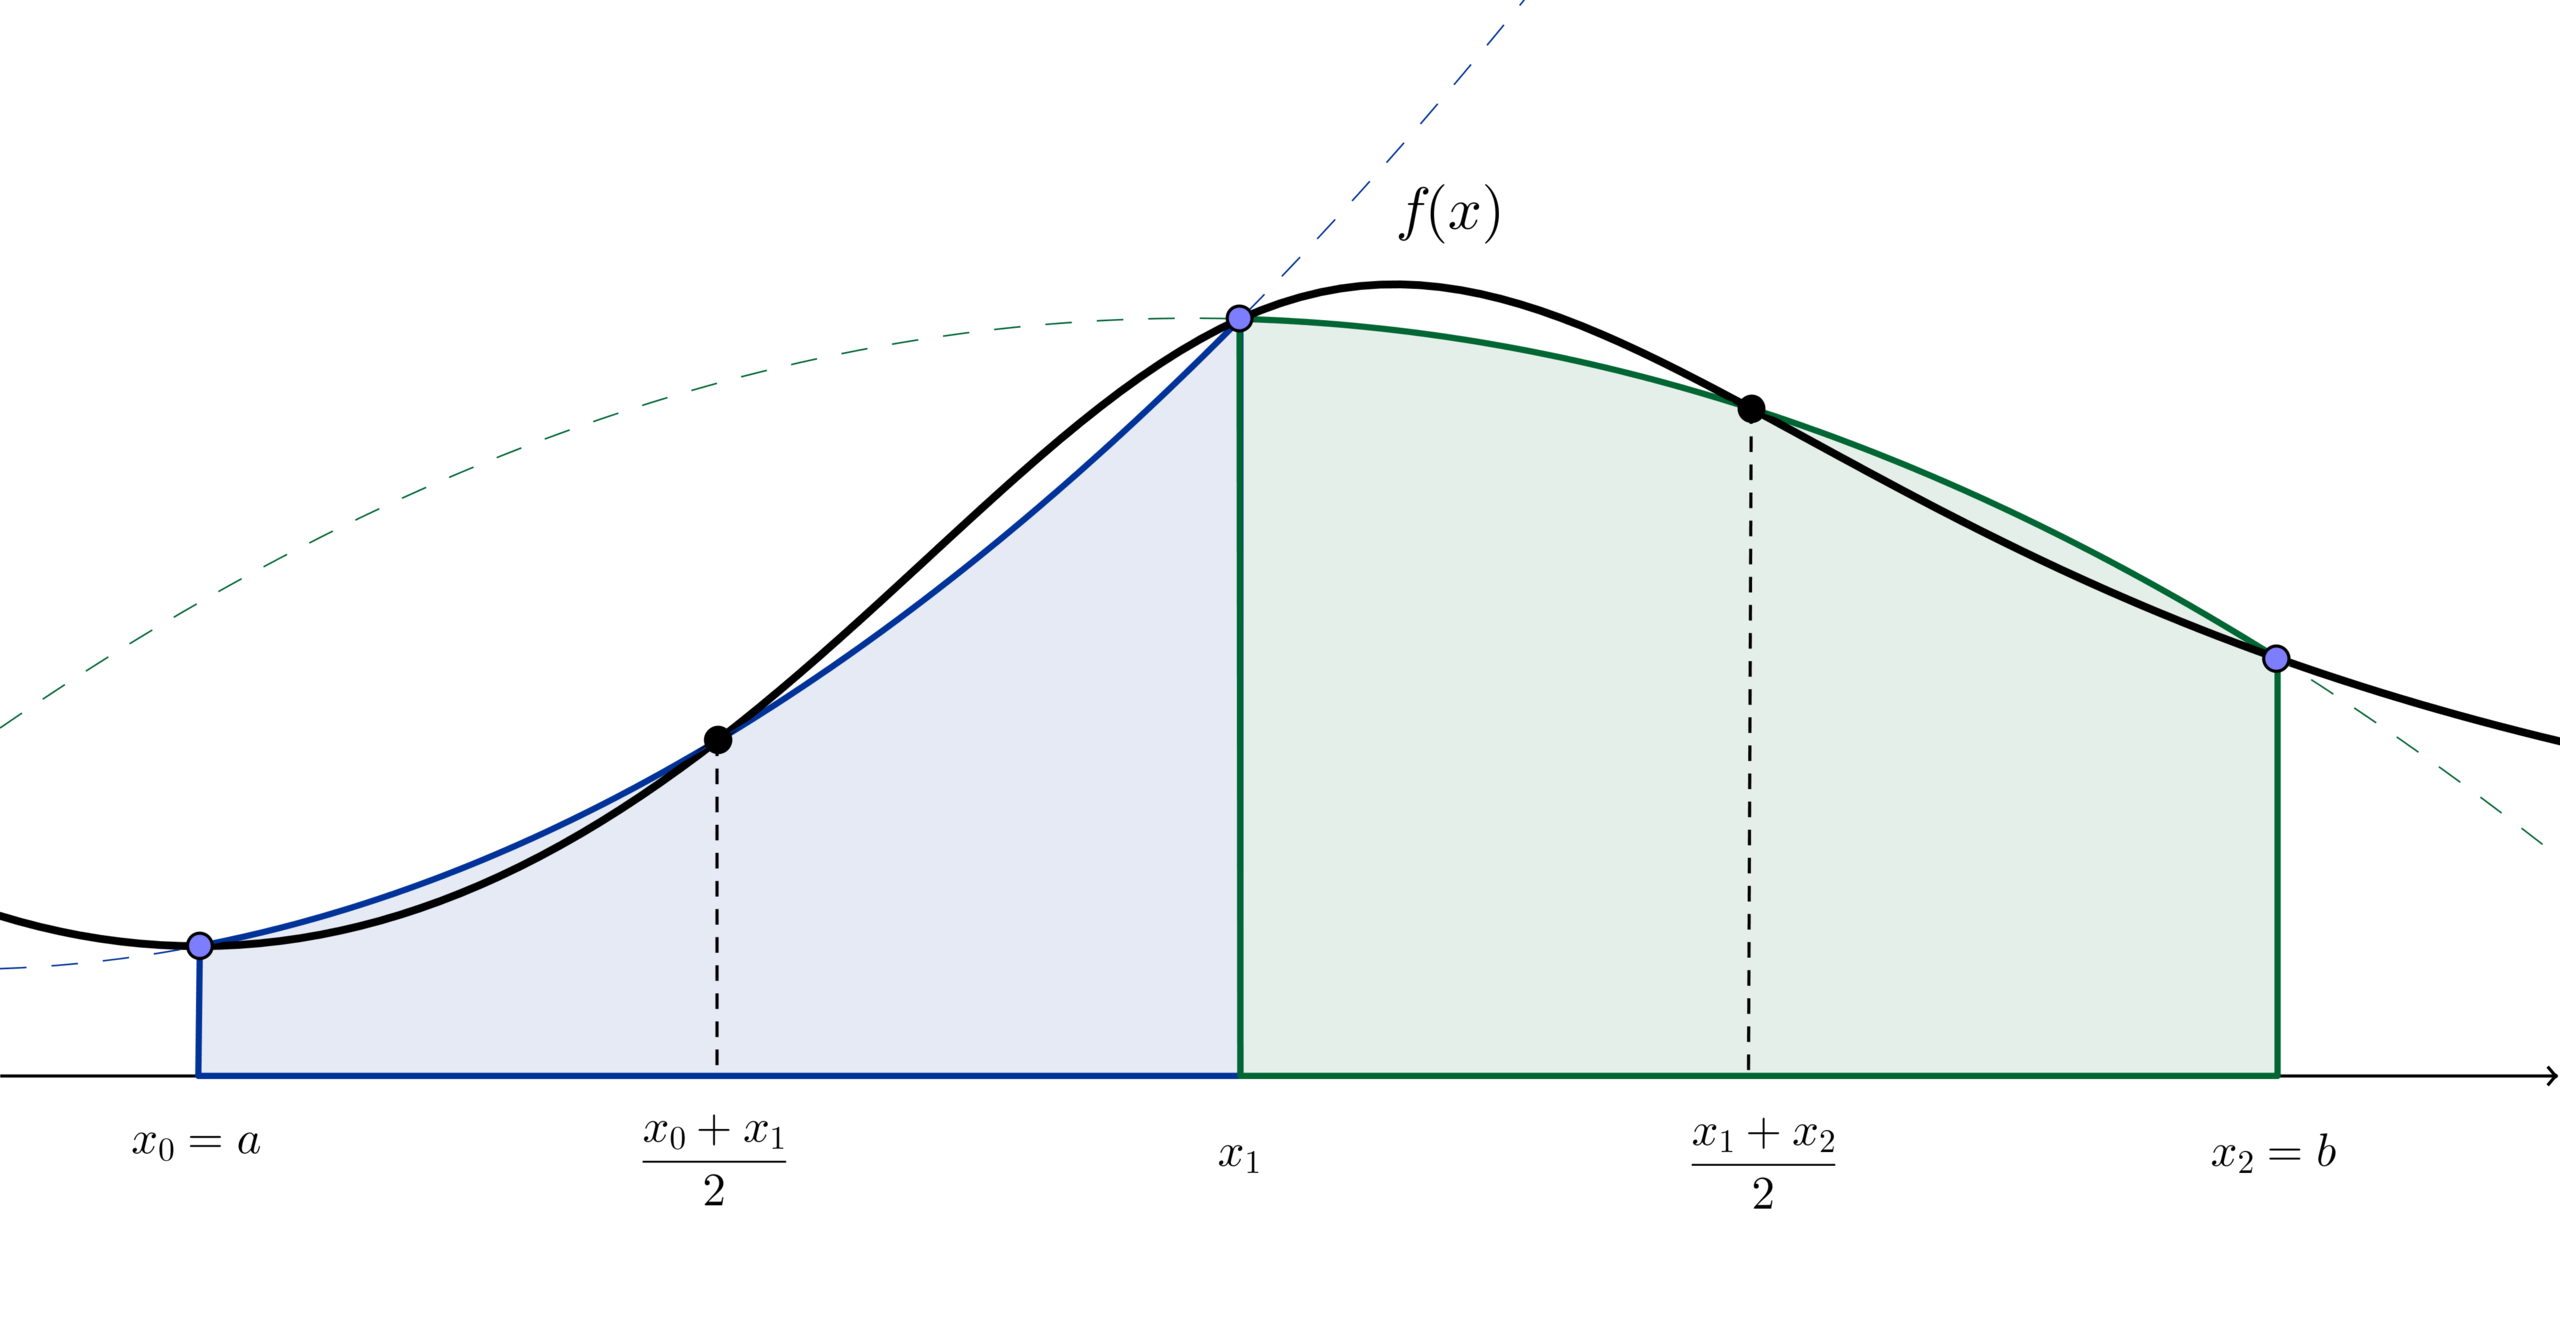
\includegraphics[width=.6\linewidth]{./titlepage.png}
		\end{figure}
		
		\vfill
		
		% Bottom of the page
		{\large \today\par}
	\end{titlepage}
	\restoregeometry
	
	\thispagestyle{firststyle}
	
	\newpage
	
	
	\tableofcontents
	\thispagestyle{general}
	\newpage

	\noindent
	Um exponentiell abfallende Funktionen auf dem unbeschränkten Intervall [0,$\infty$) zu integrieren, bieten sich zwei Möglichkeiten an
	\begin{itemize}		
	\item[a)] 	Abschneiden des unbeschränkten Intervalls und Anwendung einer Quadraturformel für ein beschränktes Intervall [0,T] für T > 0
	\item[b)] 	Anwendung einer Gaußquadratur für die Gewichtsfunktion w(x) = exp(-x) 
	\end{itemize}
	\section{Summierte Trapezformel auf einem endlichen Intervall}\label{trapez}
	\begin{mylemma}\label{lemma1.1}
	Sei $f$ : [0,$\infty$) $\rightarrow$ $\R$ eine beschränkte Funktion. Des weiteren definieren wir für eine Menge M $\subset$ [0,$\infty$) das gewichtete Integral von $f$ mit
	\begin{align*}
		Q_M(f) := \int_{M}^{}{f(x)exp(-x)dx}
	\end{align*}
	Das Integral $Q_{[0,\infty)}(f)$ kann man approximieren, indem man für ein T > 0 das Integral auf dem beschränkten Intervall $Q_{[0,T)}(f)$ durch die summierte Trapezformel $Q_{h,T}(f)$ berechnet. Es folgt eine Fehlerabschätzung der Form 
	\begin{align}
		|Q_{[0,\infty)}(f) - Q_{h,T}(f)| \le C_1\varepsilon_T + C_2T\varepsilon_h \label{eq:trapez-fehler}
	\end{align}
	wobei die Terme $\varepsilon_T, \varepsilon_h$ lediglich von $T$ bzw. $h$ abhängen und $C_1, C_2$ jeweils von $T,h$ unabhängig sind. Des weiteren wir vorausgesetzt, dass f hinreichend glatt ist und die Supremumsnorm der zweiten Ableitung der Funktion beschränkt ist.
	\end{mylemma}
	\begin{myproof}
		Mit \autocite[vgl.][40-41]{skript}: \\
		und $C_1 := \norm{f}_{\infty}$ , \quad $\varepsilon_T := e^{-T}$ ,
		\quad $C_2 := \norm{f^{''}}_{\infty}$ , \quad $\varepsilon_h := \frac{h^{2}}{12}$ folgt unmittelbar
		\begin{align*}
			|Q_{[0,\infty)}(f) - Q_{h,T}(f)| &\le |Q_{[0,\infty)}(f) - Q_{[0,T]}(f)| + |Q_{[0,T]}(f) - Q_{h,T}(f)| \\
			&= |Q_{(T,\infty)}(f)| + |Q_{[0,T)}(f) - Q_{h,T}(f)| \\
			&\le \norm{f}_{\infty}\int_{T}^{\infty}{e^{-x} dx} + \left|-\frac{T}{12}h^{2}f^{''}(\xi)\right| \\
			&= C_1e^{-T} + T\frac{h^{2}}{12}|f^{''}(\xi)| \\
			& \le C_1\varepsilon_T + \norm{f^{''}}_{\infty}T\frac{h^{2}}{12} \\
			& = C_1\varepsilon_T + C_2T\varepsilon_h 
		\end{align*}
	\end{myproof}
	\newpage
	\begin{mybeispiel}
		Es wird T fix gewählt und der Fehler in Abhängigkeit von h geplottet mit der Funktion $f(x) := \frac{sin(x)}{x}$
		\lstinputlisting[language=Python, firstline = 4, lastline = 20, caption=Implementierung des Fehlers mit fixem T]{fehlerTsinx.py}
		\begin{figure}[H]
			\begin{center}
				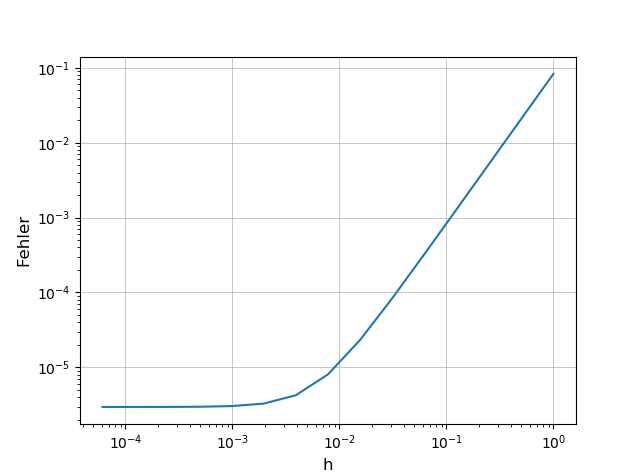
\includegraphics[width=0.8\textwidth]{FehlerplotT.png}
			\end{center}
			\caption{Fehlerplot in Abhängigkeit von h.}
			\label{fig:fehlerplott}	
		\end{figure}
		\newpage
		Um alles übersichtlicher zu machen, wird nun h fix gehalten und T variiert. 
		\lstinputlisting[language=Python, firstline = 4, lastline = 20, caption=Implementierung des Fehlers mit fixem h]{fehlerhsinx.py} 	
		\begin{figure}[H]
			\begin{center}
				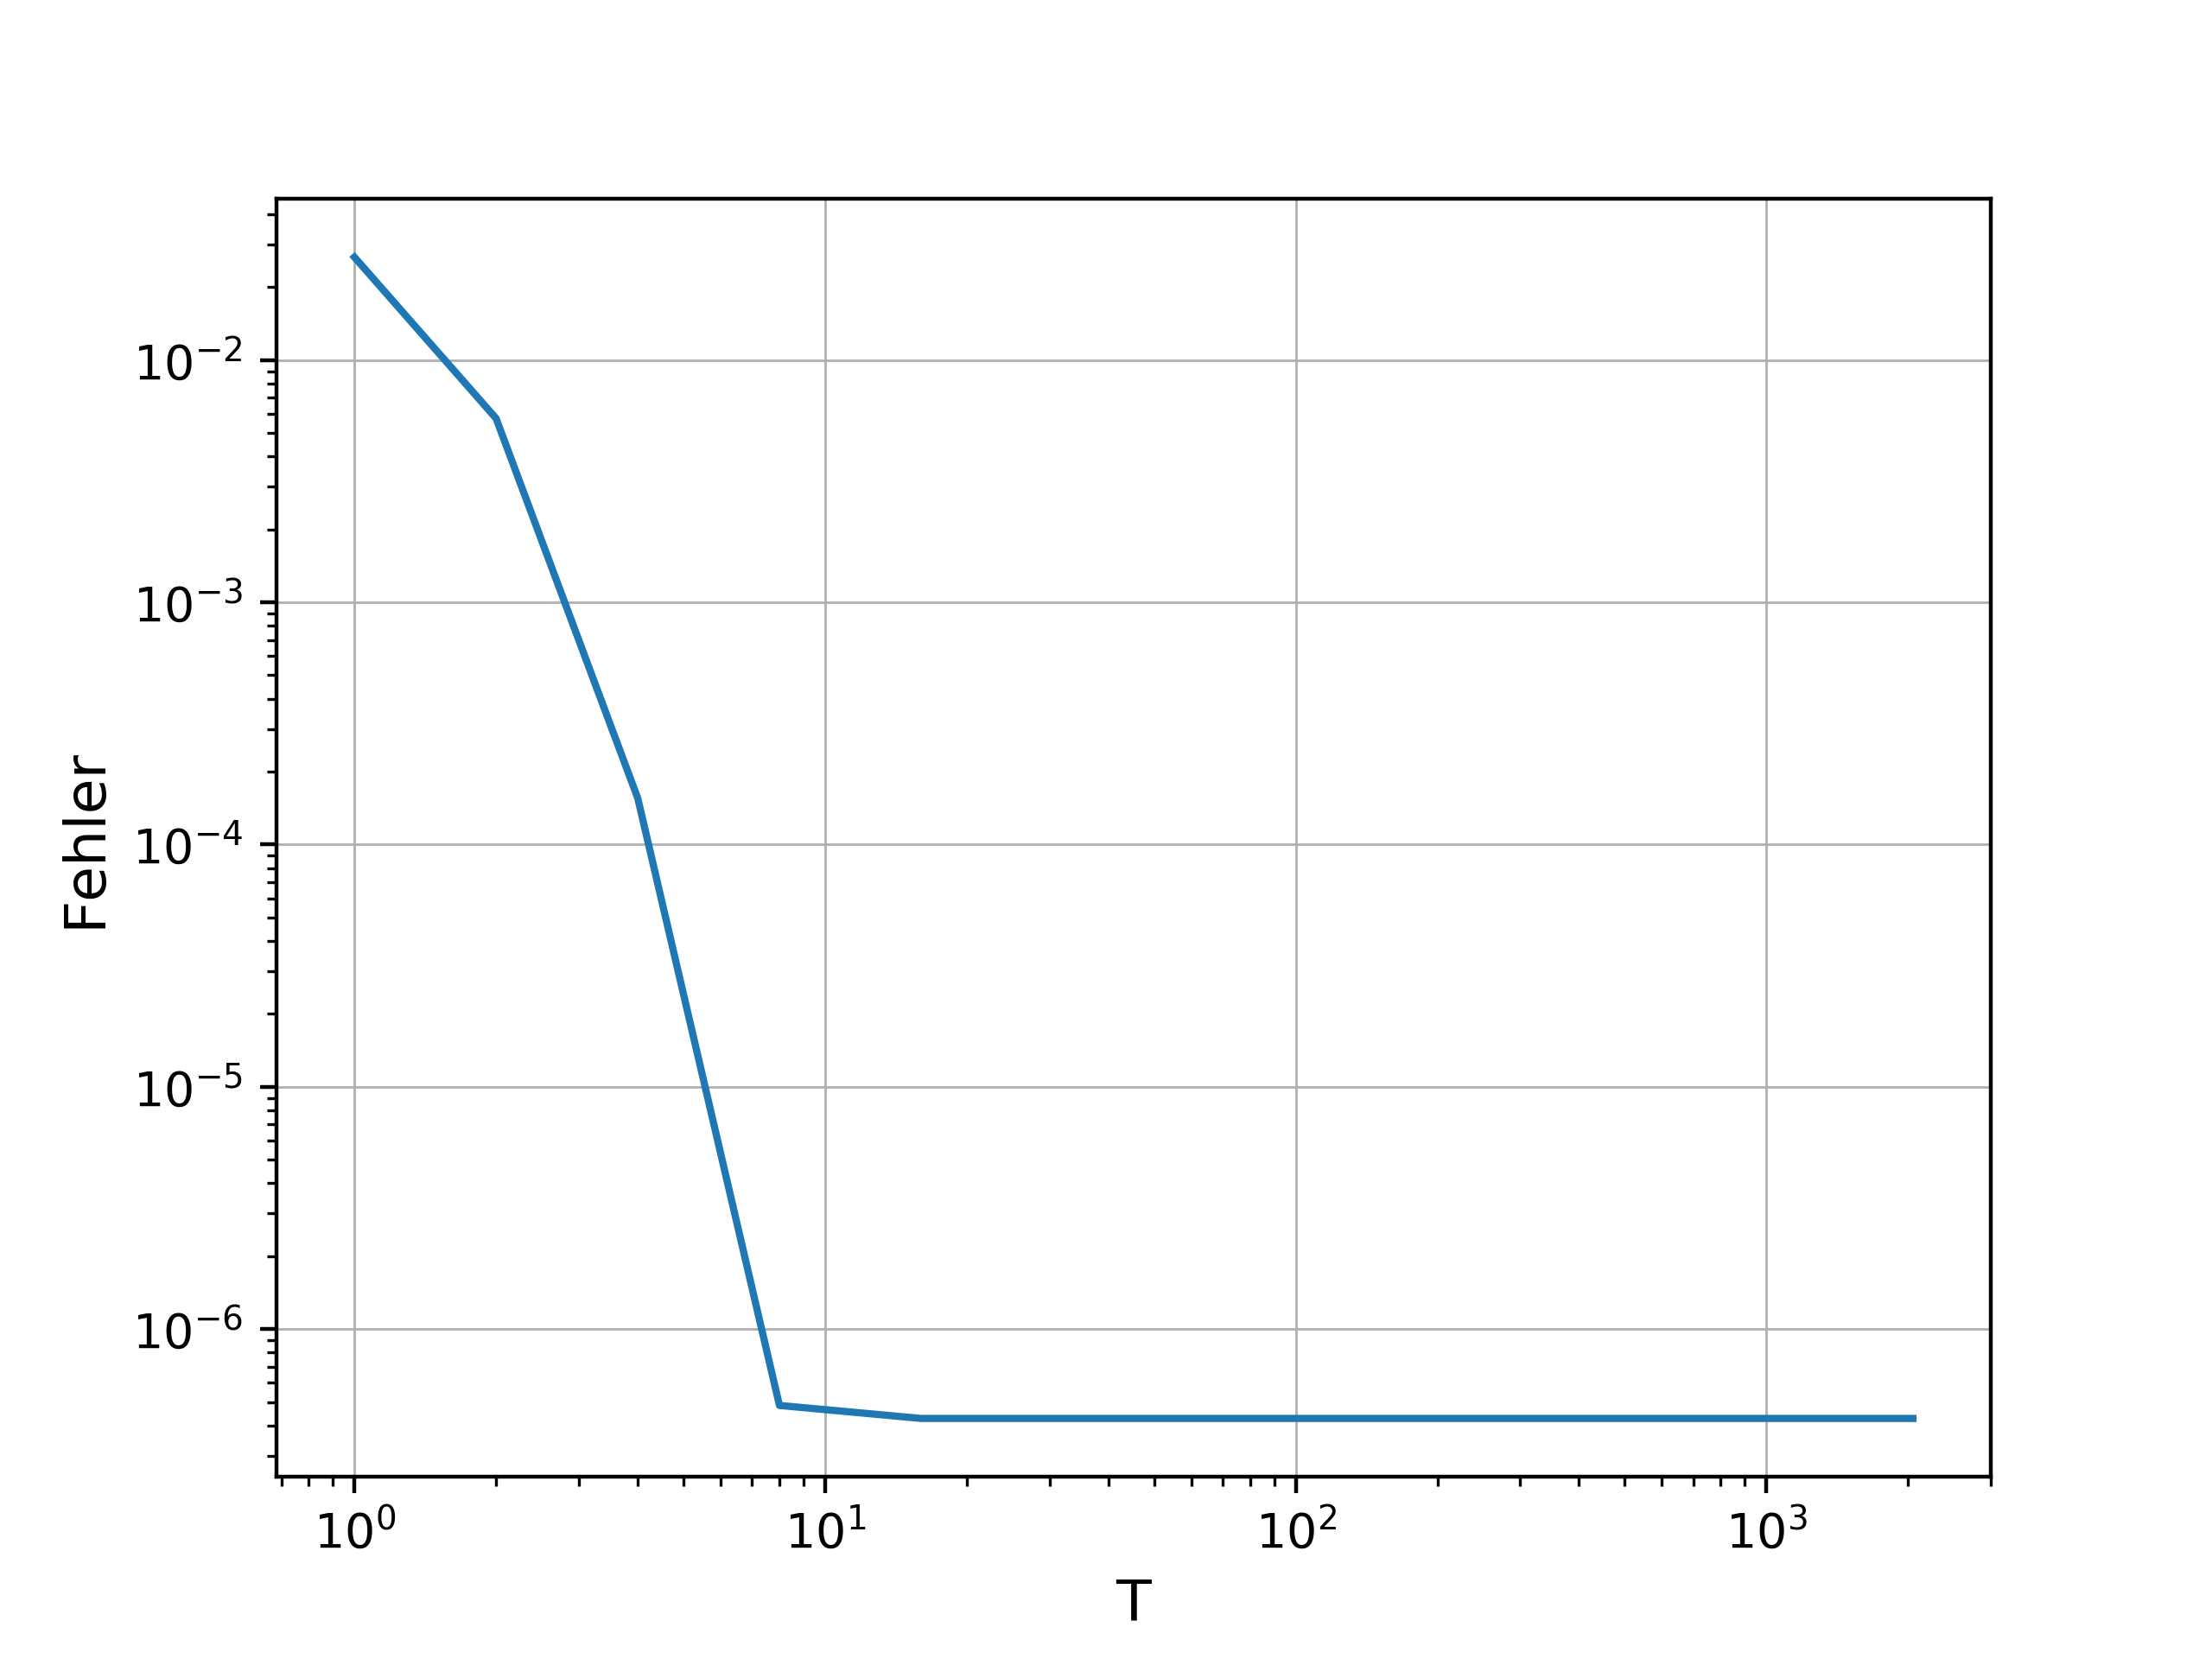
\includegraphics[width=0.8\textwidth]{Fehlerploth.png}
			\end{center}
			\caption{Fehlerplot in Abhängigkeit von T.}
			\label{fig:fehlerploth}	
		\end{figure}
		\newpage
		Man sieht nun aus \cref{fig:fehlerplott}, dass bei kleiner werdenden h sich der Fehler ab einem gewissen Wert nicht mehr ändert. Das liegt daran, dass wir das Intervall $[0,\infty]$ auf $[0,T]$ beschränken und somit auch bei Verfeinerung von h sich der Fehler nicht mehr ändert, d.h. die maximale Genauigkeit der numerischen Integration ist erreicht worden. Dasselbe passiert auch in \cref{fig:fehlerploth}, nur dass hier bei einer fixen Schrittweite, sich der Fehler ab einem gewissen T bzw. ab einem gewissem n nicht mehr ändern wird. Um das exakte Integral zu bekommen, müsste man fordern, dass h $\rightarrow $0 und T $\rightarrow \infty$ strebt, da wir aber das Intervall abschneiden und eine Quadraturformel drauf anwenden, ist die nicht möglich, und uns genügt ein minimaler Fehler. Die beiden Plot ändern sich auch bei verschieden Funktionen nicht, das einzige was passiert, ist dass sich der Punkt an dem der Fehler sich nicht mehr ändert, sich nach links oder rechts verschiebt.  \\ \newline
		\textbf{Bemerkung}: Damit der Fehler minimal ist, soll $\varepsilon_T \approx T\varepsilon_h$ gelten. D. h. bei einer gegebenen Anzahl an Funktionsauswertungen kann man T bzw. h wie im folgenden Plot gewählt. Anders angeschrieben soll also $h \approx \sqrt{\frac{12e^{-T}}{T}}$ bzw. $n \approx \sqrt{\frac{T^{3}}{12e^{-T}}}$ gelten.
		\begin{figure}[H]
			\begin{center}
				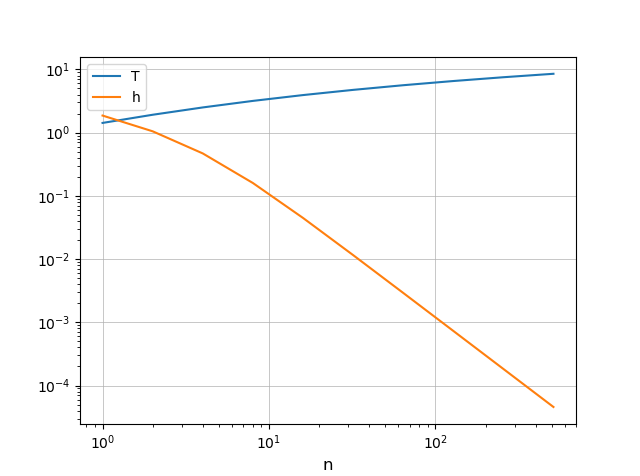
\includegraphics[width=0.8\textwidth]{parameterth.png}
			\end{center}
			\caption{Parameterwahl bei fixem n.}
			\label{fig:parameterth}	
		\end{figure}
		 
	\end{mybeispiel}
	\newpage
	
	
	
	%sebastians teil
	\section{Gau\ss-Laguerre Quadratur}\label{gauss}
	Zun\"achst  sei bemerkt, dass\autocite[45]{skript}:
	\begin{mykorollar}\label{4.15}
		Es existiert eine eindeutig bestimmte Folge $(q_n)$ von Polynomen der Form
		\begin{align*}
		q_0(x)&\coloneqq 1\\
			q_n(x)&\coloneqq x^n+r_{n-1}(x),\quad x\in [a,b]
		\end{align*}
		mit $r_{n-1}\in \prod_{n-1}$, die die Orthogonalith\"atsbeziehungen  $(q_n,q_m)_w=0,\; n\neq m $ erf\"ullen.
	\end{mykorollar}

	\noindent und
	\begin{mylemma}
		Jedes der orthogonalen Polynome $q_n\in \prod_n$, aus \cref{4.15} besitzt $n$ einfache Nullstellen in $(a,b)$.
	\end{mylemma}

	\noindent Woraus sich dann folgender Satz ergibt:
	\begin{mytheorem}\label{aufgabec-satz}
		%Korollar 4.15  \autocite[45]{skript}
		Die Orthogonalpolynome $q_n \in \prod_n$ aus \cref{4.15} sind eindeutig durch die folgenden 3 Terme gegeben
		\begin{align*}
			q_0(x) &\coloneqq 1\\
			q_1(x) &\coloneqq (x-\beta_0) q_0 = x-\beta_0 \\
			 q_{n+1}(x) &\coloneqq (x-\beta_n)q_n(x)-\gamma^2_n q_{n-1}(x) \quad \text{f\"ur}  \quad n\geq 1
		\end{align*}
		mit
		\begin{align*}
			\beta_n\coloneqq \frac{(xq_n,q_n)_w}{\norm{q_n}^2_w} \quad \text{und} \quad 
			\gamma_n\coloneqq \frac{\norm{q_n}_w}{\norm{q_{n-1}}_w}
		\end{align*}
		Weiter sind die Eigenwerte der Matrix
		\begin{align*}
		T\coloneqq 
			\begin{pmatrix}
			\beta_0 		 & 	\gamma_1 	&  						& &\\
			\gamma_1 	 & \beta_1 			& \gamma_2	  & & \\
			 				    	&  \gamma_2   & \ddots 		      & \ddots &\\
			 				    	&					& \ddots &	\beta_{n-1} & \gamma_n\\
			 				    	&	&	&\gamma_n &\beta_n&\\
			\end{pmatrix}
			\in \mathbb{R}^{(n+1)\times (n+1)}
		\end{align*}
		die Nullstellen $x_0,\dots ,x_n$ des $(n+1)$-ten Orthogonalpolynoms $q_{n+1}$ und die zugeh\"origen Gewichte der Gau\ss-Quadratur sind gegeben durch
		\begin{align*}
			\alpha_j \coloneqq \left(\frac{(v_j)_1}{\norm{v_j}_2}\right)^2 \int_{a}^{b} w(x)dx,\quad j=0,\dots,n
		\end{align*}
		wobei $(v_j)_1$ die 1.Komponente eines Eigenvektors $v_j \in \mathbb{R}^{n+1}\setminus \{0\}$ zum Eigenwert $x_j$ ist.
	\end{mytheorem}
	\begin{myproof}
		
	\end{myproof}
	\newpage
	Somit ist also die in \Cref{aufgabed-code-main,aufgabed-code-gauss} zu sehende Vorgehensweise gerechtfertigt.
	\lstinputlisting[language=c,firstline=17,lastline=20,label={aufgabed-code-main},caption={M\"ogliche Implementierung von \cref{aufgabec-satz} - main.cpp}]{../code/aufgabe-d/main.cpp}
	\lstinputlisting[language=c,firstline=13,lastline=49,label={aufgabed-code-gauss},caption={gauss.cpp}]{../code/aufgabe-d/gauss.cpp}
	
	\begin{figure}[H]
		\begin{center}
			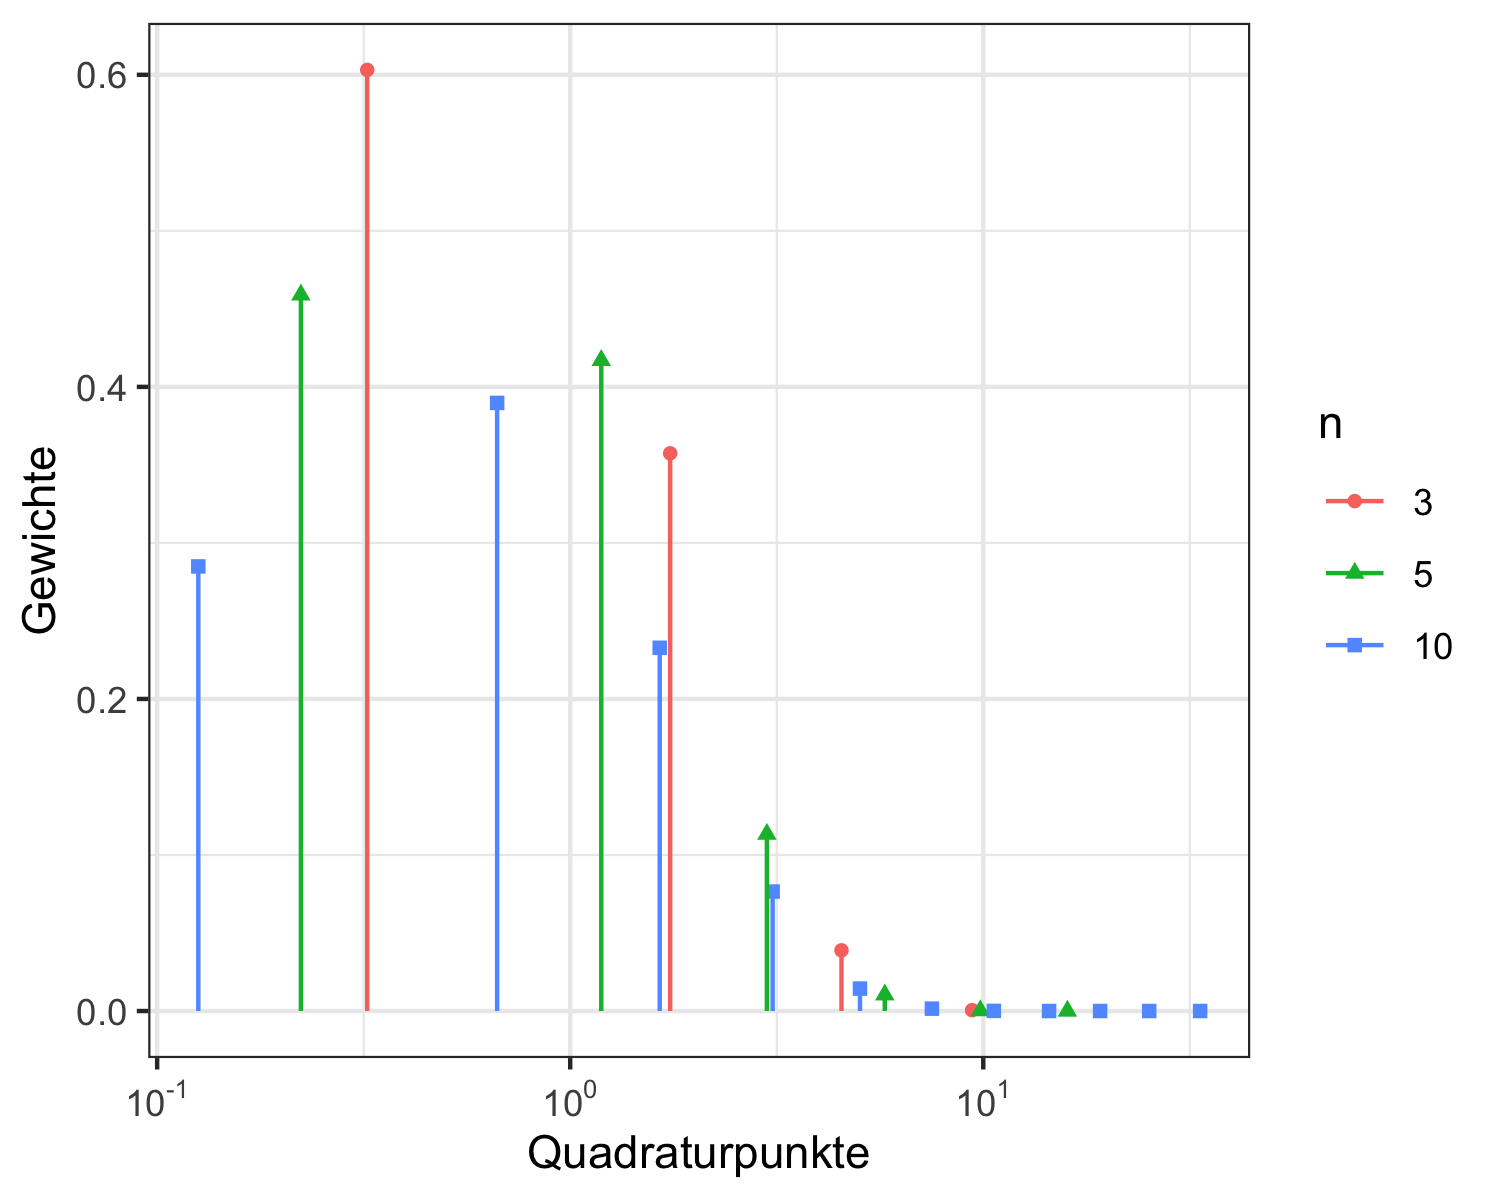
\includegraphics[width=0.8\textwidth]{../plots/quadraturpunkte-n-zusammen.png}
		\end{center}
		\caption{Quadraturpunkte und zugeh\"orige Gewichte}
		\label{fig:quadraturpunkte}
	\end{figure}
	
	\newpage
	\section{Vergleich der Methoden aus \cref{trapez,gauss}}
	%Bei der summierten Trapezformel wurde für jedes n ein optimales T gewählt wie in \cref{fig:parameterth}
	F\"ur die Funktionen $f:[0,\infty)\mapsto \mathbb{R},f(x)=\frac{1}{e^x+7}$ und $\omega:[0,\infty)\mapsto \mathbb{R},\omega(x)=e^{-x}$, konvergiert die Gauss-Laguerre Quadratur wesentlich schneller gegen $\int_{0}^{\infty}f(x)\omega(x)dx$ als die in \cref{trapez} beschriebene Integrationsmethode.(\cref{fig:vergleich})
	\begin{figure}[H]
		\begin{center}
			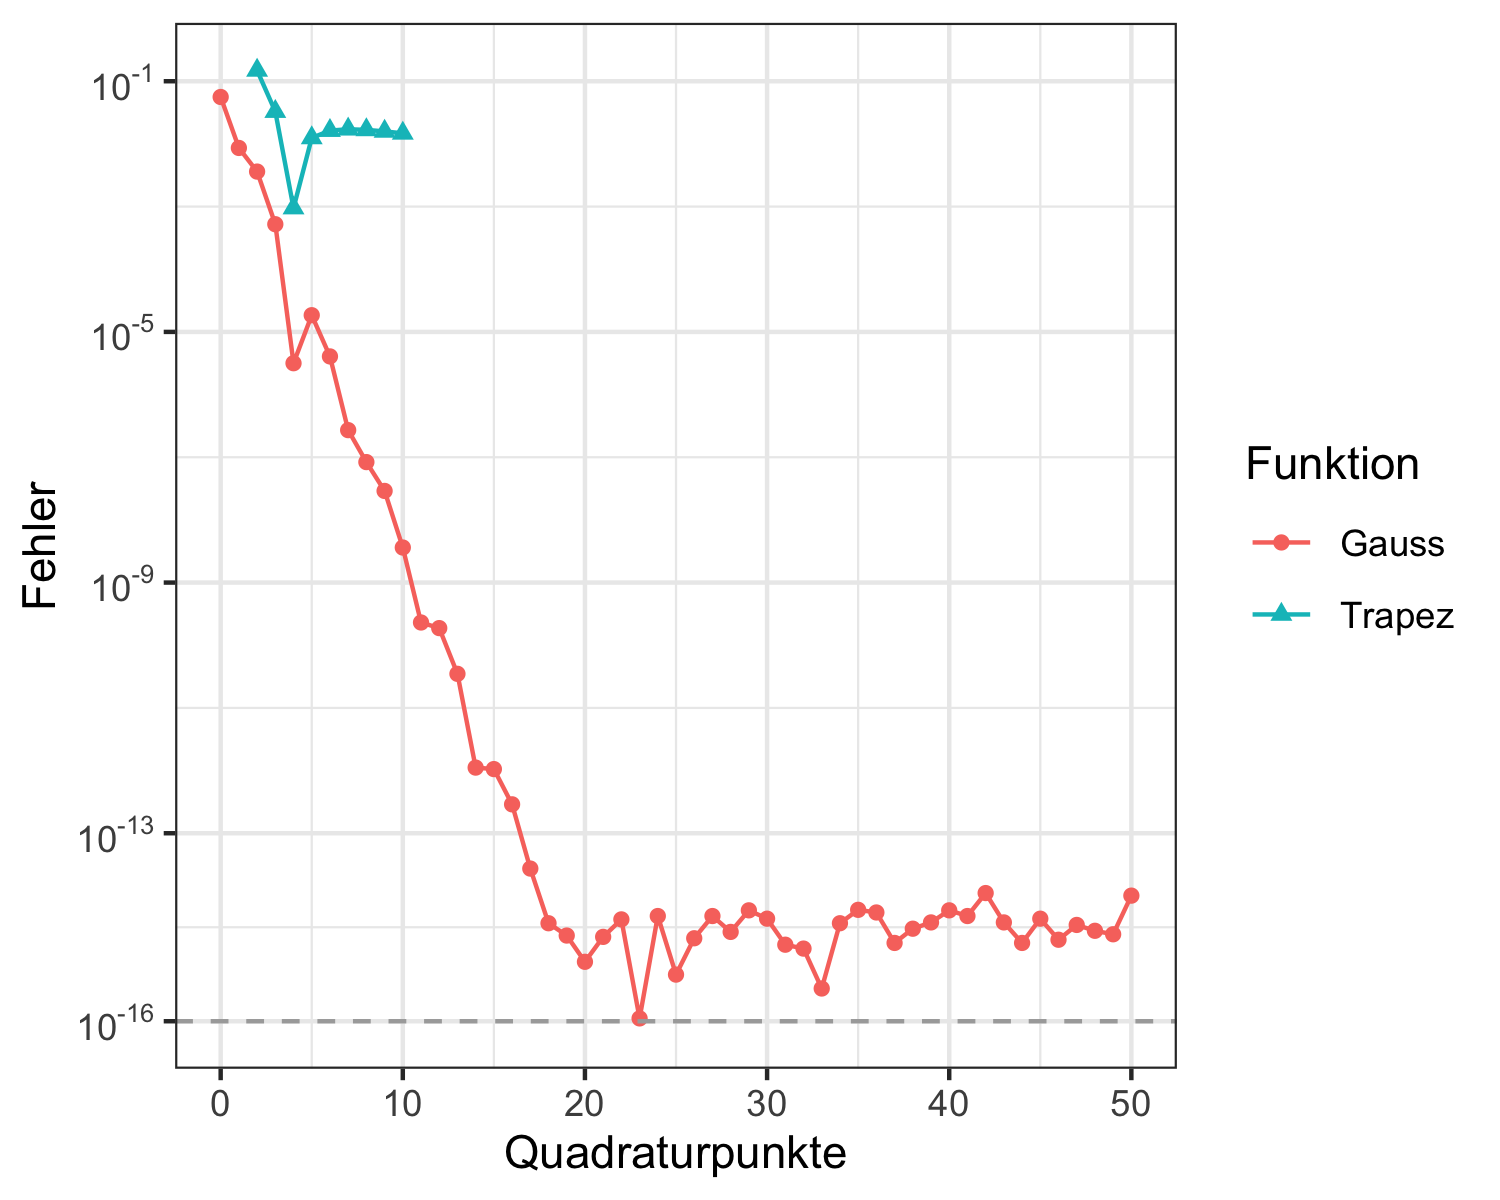
\includegraphics[width=0.8\textwidth]{../plots/aufgabe-e2.png}
		\end{center}
		\caption{Vergleich der Integrationsmethoden aus \cref{gauss,trapez}}
		\label{fig:vergleich}	
	\end{figure}


	\subsection{Beschleunigung der Konvergenz}
	Da f\"ur Funktionen $f,g$, die auf dem Intervall $[a,b]$ Riemann-integrierbar sind gilt \autocite[vgl.][271]{ana2}: 
	\begin{align*}
		f(x)\leq g(x): x \in [a,b]\Rightarrow \int_{a}^{b}f(x)dx \leq \int_{a}^{b}g(x)dx,
	\end{align*}
	ergibt sich f\"ur den Fehler $C_1\varepsilon_T$ aus \cref{eq:trapez-fehler} f\"ur andere Gewichtsfunktionen $\omega : f(x)\omega(x) \leq f(x)e^{-x}, x \in [T,\infty)$
	\begin{align*}
		\abs{\int_{0}^{\infty}f(x)e^{-x}dx-\int_{0}^{T}f(x)e^{-x}dx} = \abs{\int_{T}^{\infty}f(x)e^{-x}dx} \geq \\
		 \abs{\int_{T}^{\infty}f(x)\omega(x)dx} =  \abs{\int_{0}^{\infty}f(x)\omega(x)dx-\int_{0}^{T}f(x)\omega(x)dx}
	\end{align*}	
	Der bei \cref{trapez} durch das Abschneiden des Intervalls $[0,\infty)$ entstehende Fehler ist also stark von der Wahl der Gewichtsfunktion abh\"angig.(\cref{fig:f-vergleich-int}) 
	Durch die Wahl einer geeigneten Gewichtsfunktion kann die Konvergenz des Integrationsverfahrens also beschleunigt werden.
	
	
	\begin{figure}[H]
		\begin{subfigure}[t]{0.5\textwidth}
			
			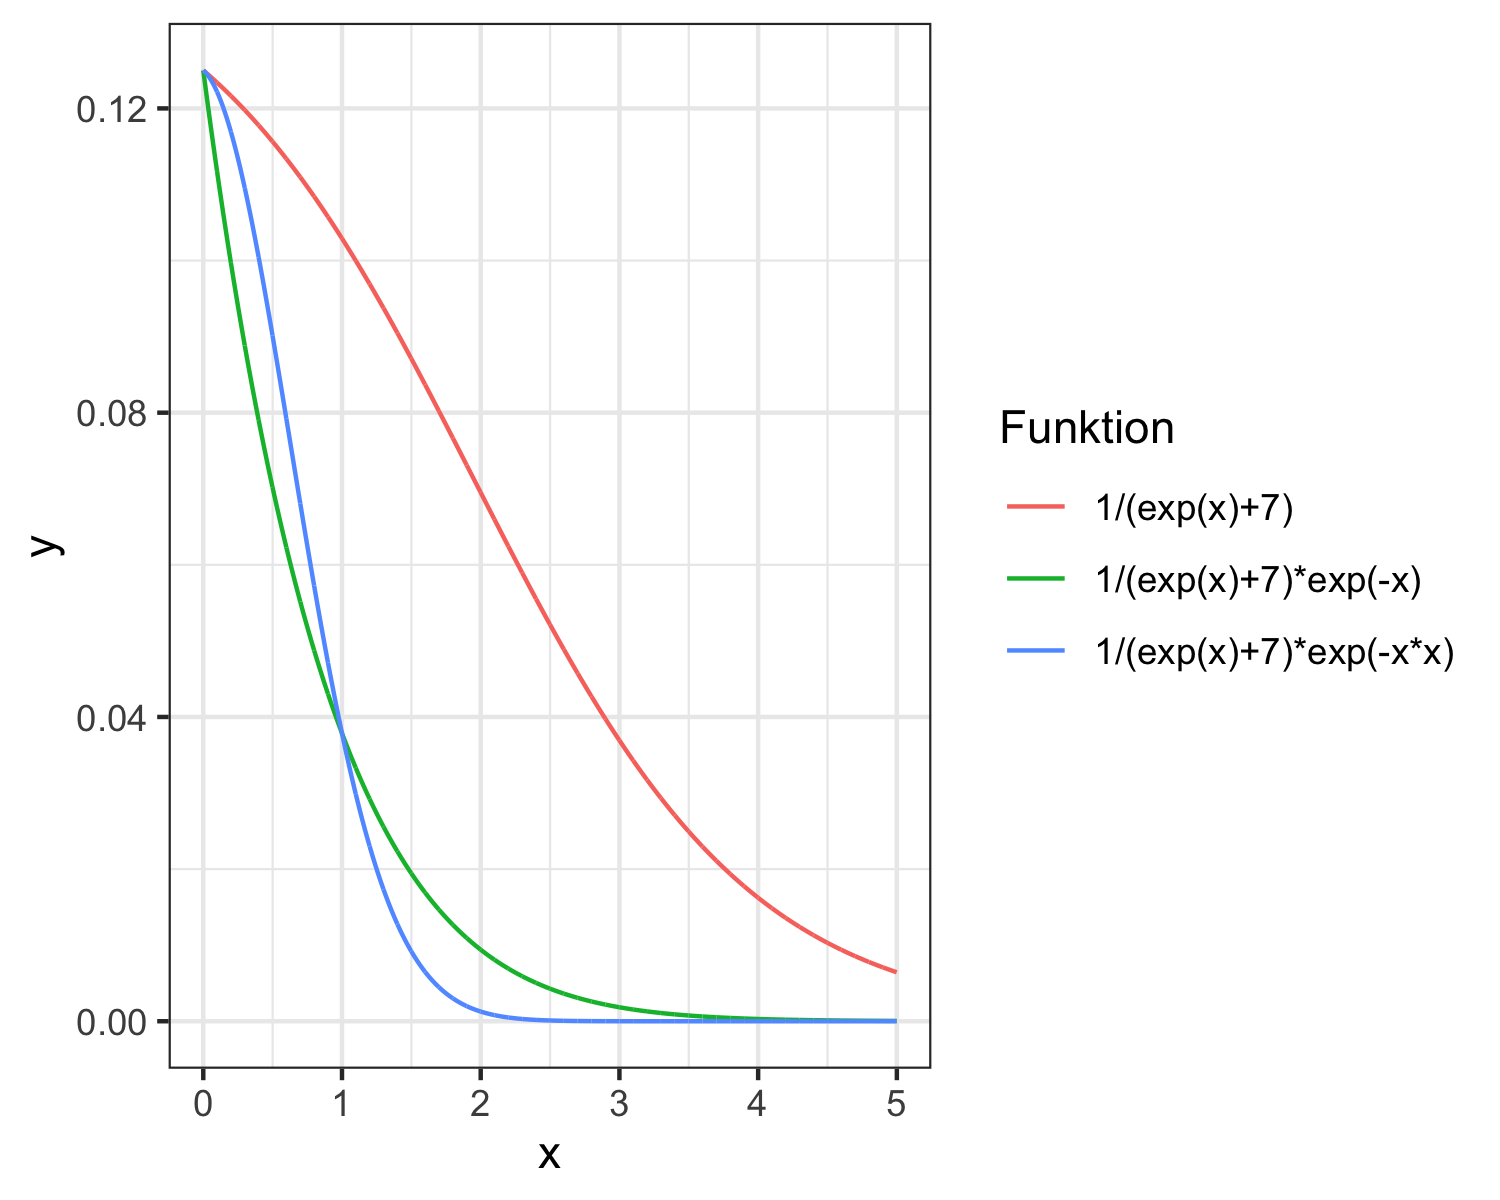
\includegraphics[width=\linewidth]{../plots/aufgabe-e-vergleich.png}
			\subcaption{$f(x)\omega(x)$ f\"ur verschiedene $\omega(x)$}\label{fig:f-vergleich}
			
		\end{subfigure}
		\begin{subfigure}[t]{0.5\textwidth}
			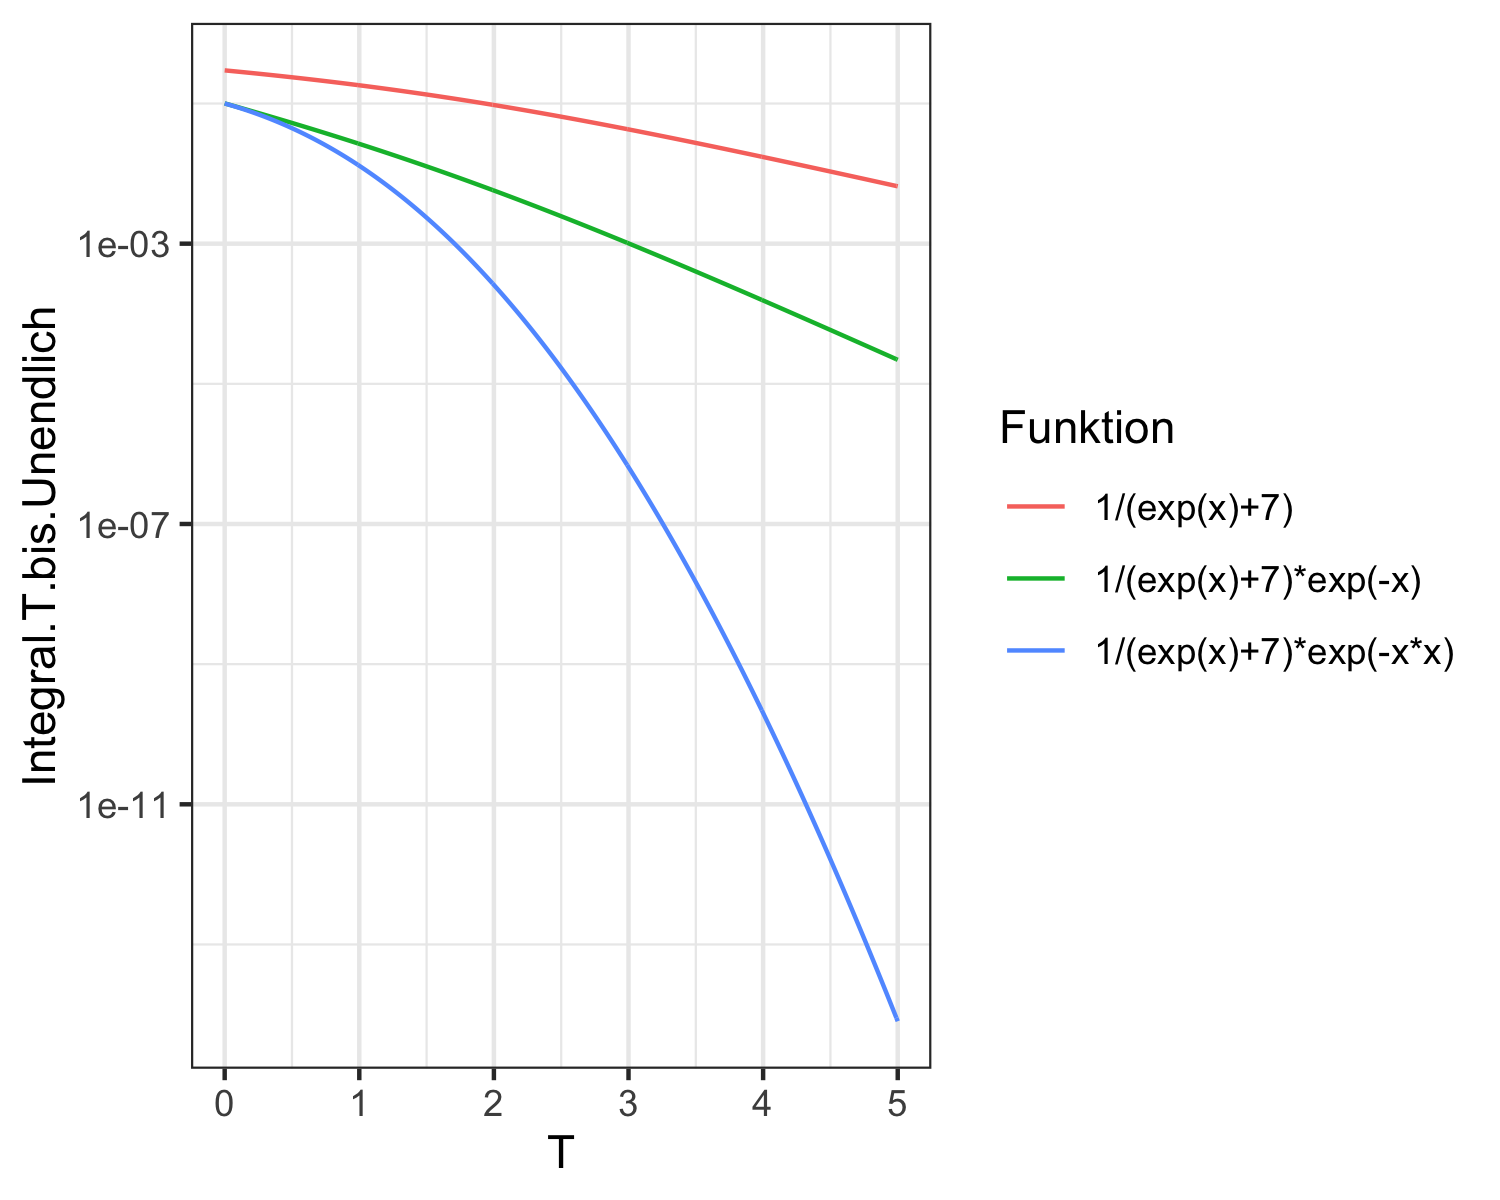
\includegraphics[width=\linewidth]{../plots/aufgabe-e-vergleich-integral.png}
			\subcaption{Von T abh\"angiger Fehler f\"ur verschiedene Gewichtsfunktionen}\label{fig:f-vergleich-int}
		\end{subfigure}
		\caption{Vergleich verschiedener Gewichtsfunktionen}
	\end{figure}

\begin{bemerkung}
	Um, wie in \cref{fig:f-vergleich-int}, mithilfe von \cref{gauss} auch Integrale der Form $\int_{a}^{\infty}f(x)\omega(x)dx:a>0$ zu berechnen kann f\"ur Funktionen $f,\omega:\int_{0}^{\infty}f(x)\omega(x)dx<\infty$ wegen \autocite[vgl.][278]{ana2}
	\begin{align*}
		\int_{a}^{\infty}f(x)\omega(x)dx = \int_{0}^{\infty}f(x+a)\omega(x+a)dx = \int_{0}^{\infty}f(x+a)\omega(x+a)\omega^{-1}(x)\omega(x)dx
	\end{align*}
	eine neue Funktion $g$ mit $g(x) \coloneqq f(x+a)\omega(x+a)\omega^{-1}(x)$ definiert werden f\"ur die gilt:
	\begin{align*}
		\int_{a}^{\infty}f(x)\omega(x)dx = \int_{0}^{\infty}g(x)\omega(x)dx \approx  \sum_{i=1}^{n}w_ig(x_i).
	\end{align*}
	Weiters k\"onnen wegen $\int_{a}^{b}f(x)\omega(x)dx = \int_{a}^{c}f(x)\omega(x)dx - \int_{b}^{c}f(x)\omega(x)dx$ f\"ur $0\leq a\leq b\leq c$ auch Integrale der Form $\int_{a}^{b}f(x)\omega(x)dx$ berechnet werden.
\end{bemerkung}
	
	
	
	\begin{figure}[H]
		\begin{subfigure}[c]{0.5\textwidth}
			
			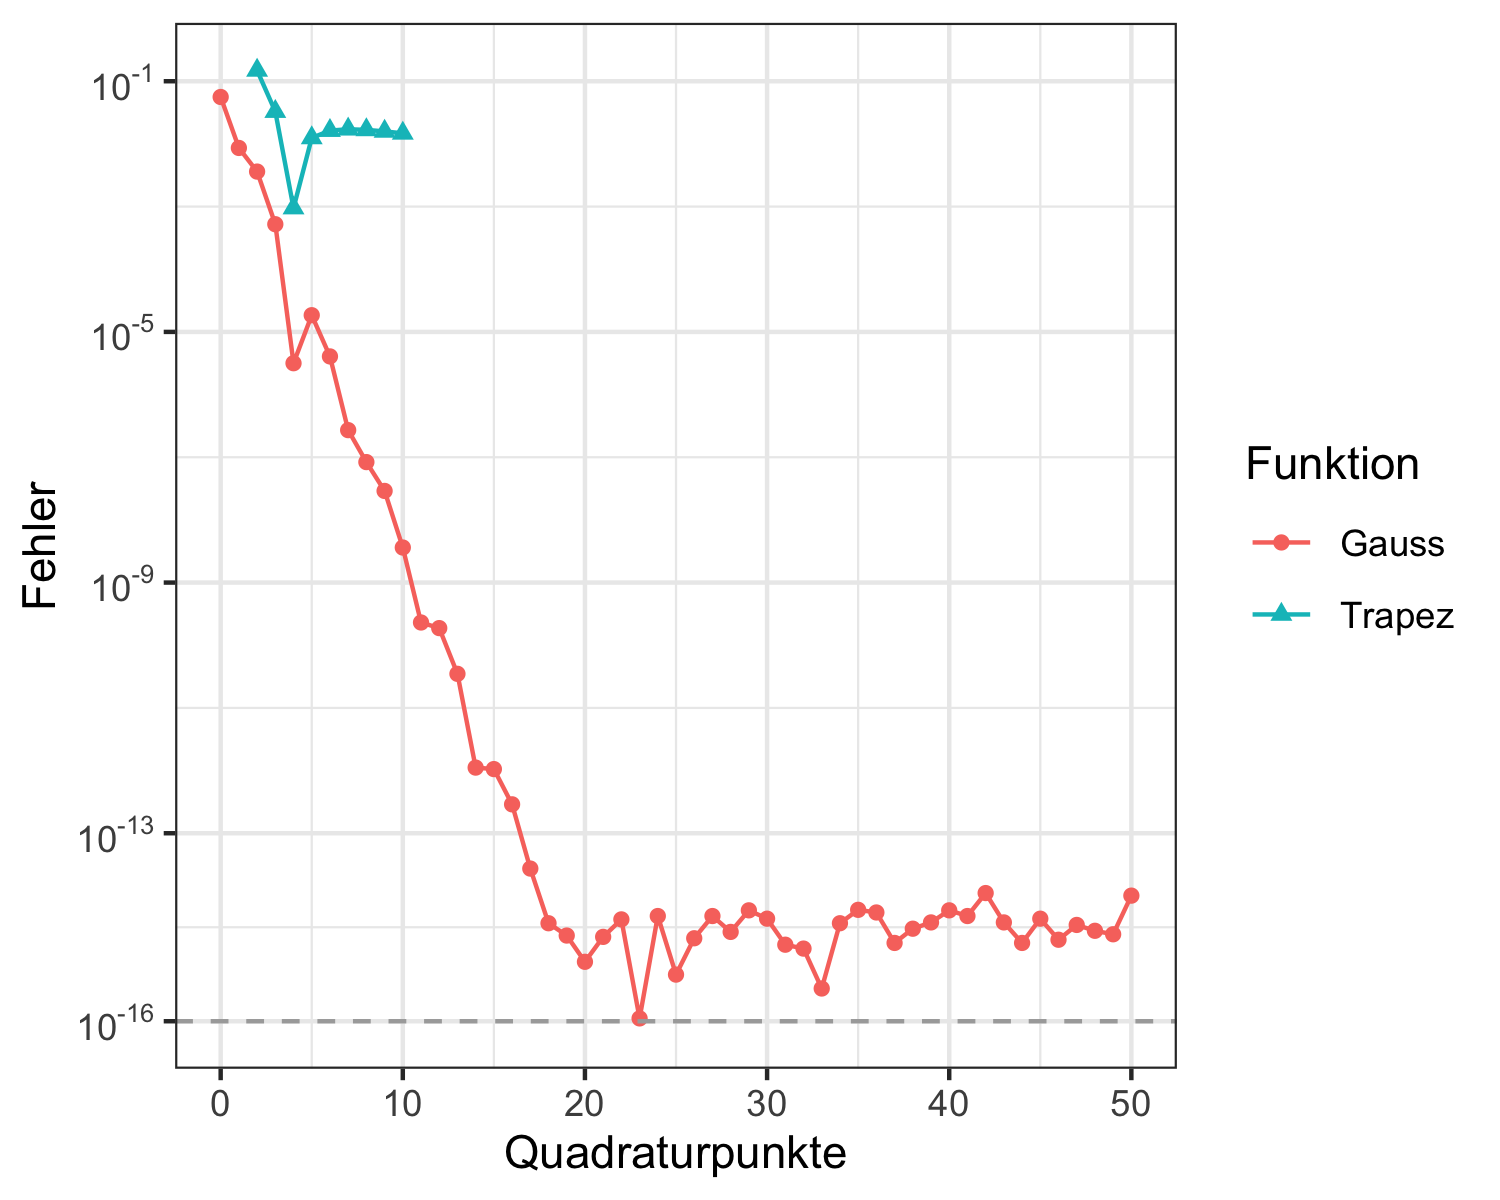
\includegraphics[width=\linewidth]{../plots/aufgabe-e2.png}
			\subcaption{Verschiedene Gewichtsfunktionen}\label{fig:gewichtsfunktionen-vergleich}
			
		\end{subfigure}
		\begin{subfigure}[c]{0.5\textwidth}
			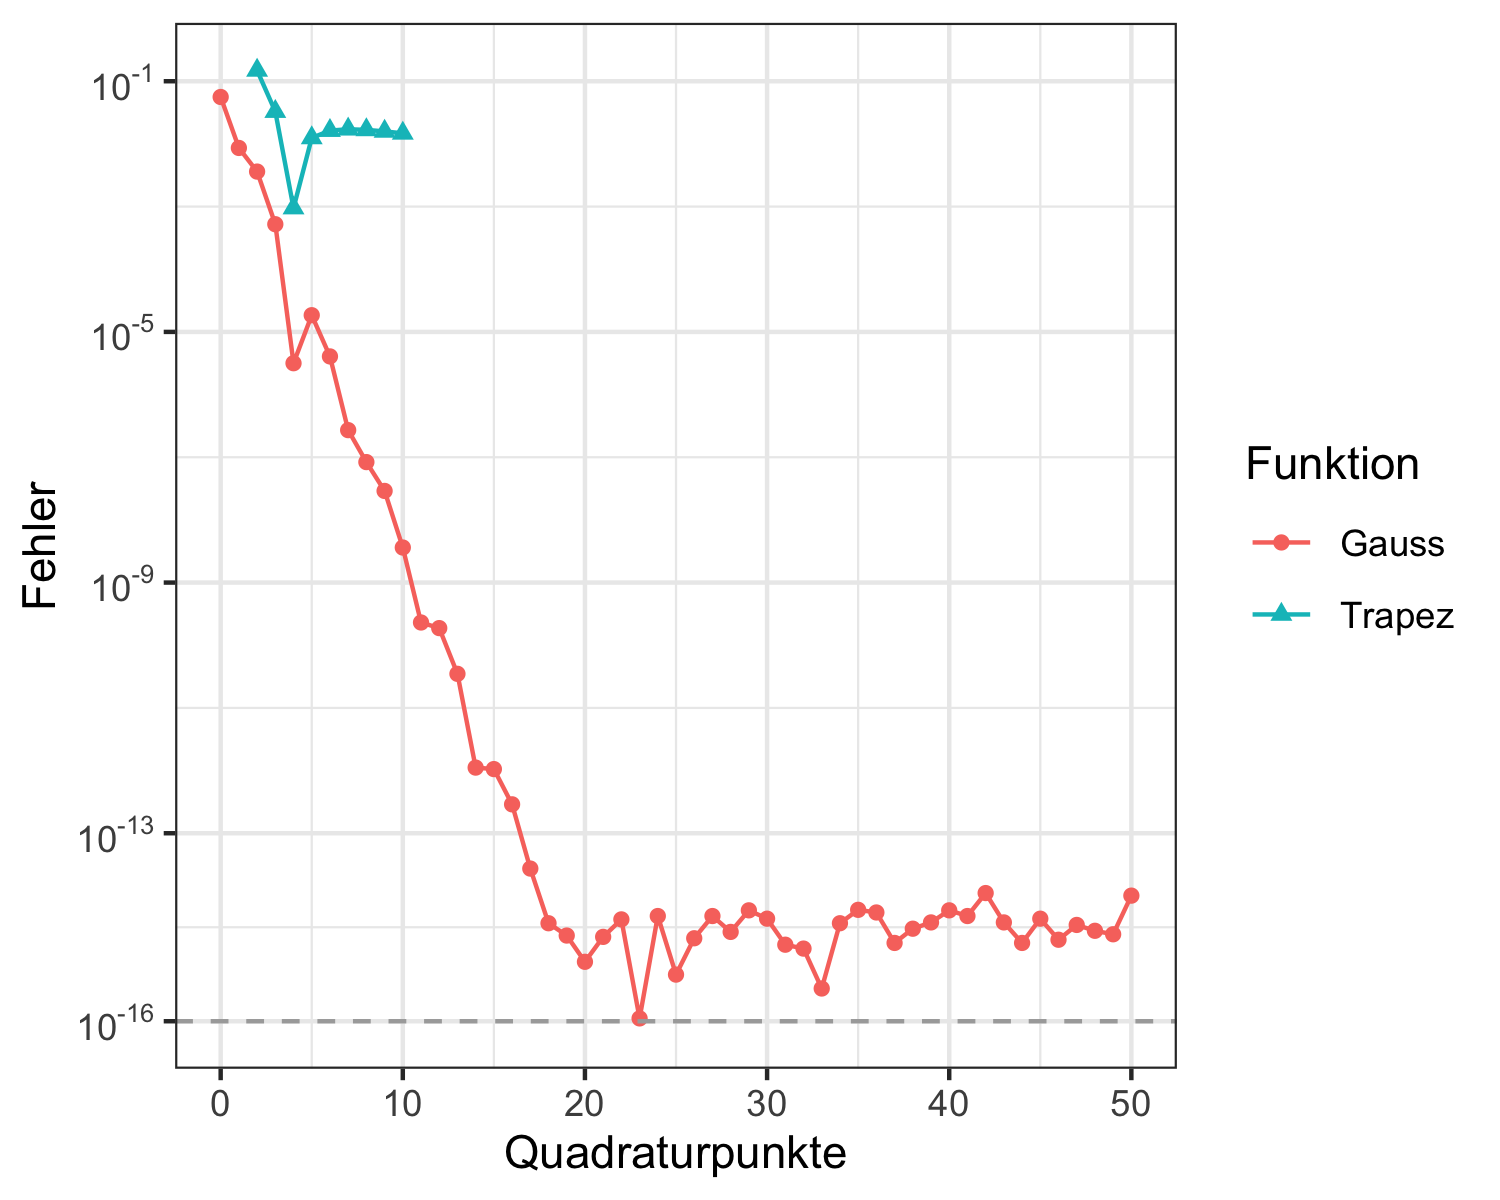
\includegraphics[width=\linewidth]{../plots/aufgabe-e2.png}
			\subcaption{Trapez vs Gau\ss quadratur}\label{fig:gauss-vs-besseretrapez}
		\end{subfigure}
	\caption{\"Anderungen zur Konvergenzbeschleunigung}
	\end{figure}
	%abbildung trapez e^-x vs e^-x^2
	
	%und abbildung trapez e^-x^2 vs gauss
	Wie in \cref{fig:gewichtsfunktionen-vergleich} zu sehen ist, geht der Fehler f\"ur $e^{-x^2}$ wesentlich schneller gegen Null als bei $e^{-x}$. Trotzdem bleibt die Konvergenz langsamer als bei der in \cref{gauss} beschriebenen Gau\ss -Quadratur (\cref{fig:gauss-vs-besseretrapez}).


	%\section{Gauss–Hermite Quadratur?}
	 % Um auch uneigentliche Integrale von $-\infty$ bis $\infty$ zu berechnen, kann als Gewichtsfunktion $e^{-x^2}$ verwendet werden. Es gilt:
	 % \begin{align*}
	%  	\int_{-\infty}^{\infty}e^{-x^2}f(x)dx \approx \sum_{i=1}^{n}w_if(x_i)
	 % \end{align*}
	%literatur,abbildungsverzeichnis etc.
	\newpage
	\printbibliography
	\listoffigures
	\thispagestyle{firststyle}
	
\end{document}

